\documentclass[tikz, border=10pt]{standalone}
\usepackage[T1]{fontenc}
\usepackage[utf8]{inputenc}
\usepackage{lmodern}
\usepackage[table]{xcolor}
\definecolor{IntelBlue}{HTML}{0068B5}
\definecolor{IntelLightBlue}{HTML}{DDEEF9}
\definecolor{FpgaOrange}{HTML}{E67E22}
\definecolor{FpgaLight}{HTML}{FDEBD0}
\definecolor{HpsGreen}{HTML}{1A7A4A}
\definecolor{HpsLight}{HTML}{D5F5E3}
\definecolor{GrayBg}{HTML}{F2F3F4}
\definecolor{GrayBorder}{HTML}{AAB7B8}
\definecolor{PassGreen}{HTML}{D5F5E3}
\definecolor{PassGreenDark}{HTML}{1E8449}
\definecolor{RowAlt}{HTML}{F7F9FB}
\definecolor{SummaryBg}{HTML}{EBF5FB}
\definecolor{NodeFill}{HTML}{D6EAF8}
\definecolor{NodeBorder}{HTML}{1B4F72}
\definecolor{InitFill}{HTML}{E5E7E9}
\definecolor{InitBorder}{HTML}{717D7E}
\definecolor{SleepFill}{HTML}{FEF5E7}
\definecolor{SleepBorder}{HTML}{935116}
\definecolor{MsgFill}{HTML}{D1F2EB}
\definecolor{MsgBorder}{HTML}{0E6655}
\definecolor{TimeoutRed}{HTML}{C0392B}
\definecolor{BtnBlue}{HTML}{1A5276}
\definecolor{ArrowGray}{HTML}{717D7E}
\usepackage{tikz}
\usetikzlibrary{shapes.geometric, arrows.meta, positioning, fit, backgrounds, calc, decorations.pathreplacing, bending, shadows.blur}
\begin{document}
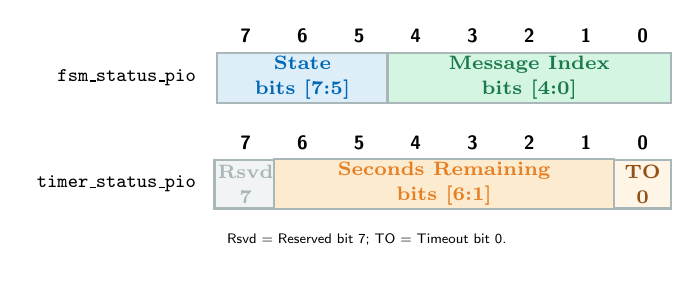
\begin{tikzpicture}[
  bitbox/.style={rectangle, draw=GrayBorder, line width=0.8pt,
                 minimum height=0.62cm, align=center, font=\scriptsize\bfseries,
                 inner sep=1.2pt},
  bitnum/.style={font=\scriptsize\bfseries\sffamily, fill=white,
                 inner sep=0.6pt},
  reglbl/.style={font=\scriptsize\bfseries, anchor=east},
]
\def\bitw{0.72}
\def\rowgap{1.35}
\foreach \b in {0,...,7} {
  \node[bitnum] at ({(7-\b+0.5)*\bitw},0.53) {\b};
}
\node[reglbl] at (-0.15,0) {\texttt{fsm\_status\_pio}};
\node[bitbox, fill=IntelLightBlue, text=IntelBlue, minimum width={3*\bitw cm}]
  at ({1.5*\bitw},0) {State\\[1pt]bits [7:5]};
\node[bitbox, fill=HpsLight, text=HpsGreen, minimum width={5*\bitw cm}]
  at ({5.5*\bitw},0) {Message Index\\[1pt]bits [4:0]};

\foreach \b in {0,...,7} {
  \node[bitnum] at ({(7-\b+0.5)*\bitw},-0.82) {\b};
}
\node[reglbl] at (-0.15,-\rowgap) {\texttt{timer\_status\_pio}};
\node[bitbox, fill=GrayBg, text=GrayBorder, minimum width={1*\bitw cm}]
  at ({0.5*\bitw},-\rowgap) {Rsvd\\[1pt]7};
\node[bitbox, fill=FpgaLight, text=FpgaOrange, minimum width={6*\bitw cm}]
  at ({4.0*\bitw},-\rowgap) {Seconds Remaining\\[1pt]bits [6:1]};
\node[bitbox, fill=SleepFill, text=SleepBorder, minimum width={1*\bitw cm}]
  at ({7.5*\bitw},-\rowgap) {TO\\[1pt]0};
\node[font=\tiny\sffamily, anchor=west] at (0,-2.05)
  {Rsvd = Reserved bit 7; TO = Timeout bit 0.};
\end{tikzpicture}
\end{document}
